\subsection{ParSplice Keyspace Analysis}
\label{sec:parsplice-keyspace-analysis}

\begin{figure}[t]
\noindent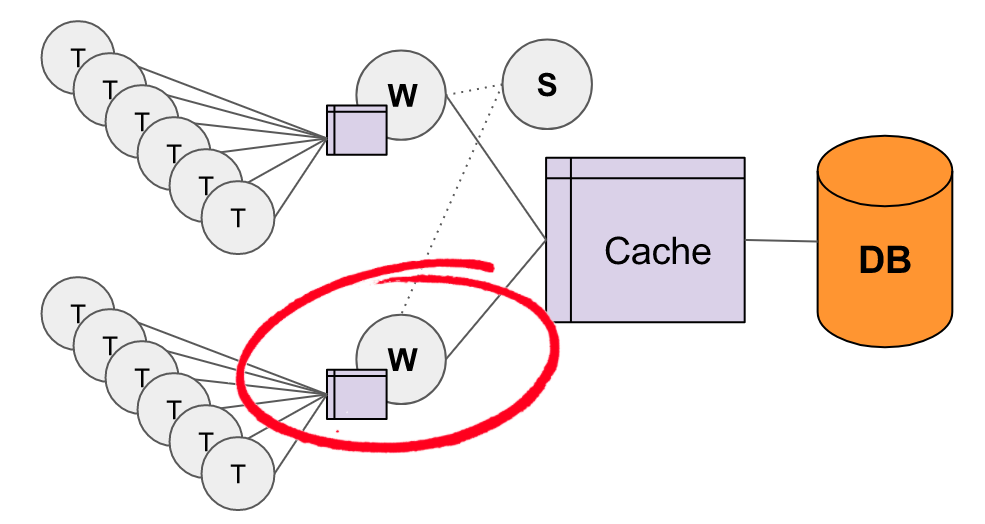
\includegraphics[width=0.5\textwidth]{./chapters/controlplane/parsplice/figures/parsplice.png}\\
\caption{The ParSplice architecture has a storage hierarchy of caches (boxes) and a
dedicated cache process (large box) backed by a persistent database (DB). A splicer
(S) tells workers (W) to generate segments and workers employ tasks (T) for more
parallelization. We focus on the worker's cache (circled), which facilitates
communication and segment exchange between the worker and its tasks.
\label{fig:parsplice}}
\end{figure}

ParSplice~\cite{perez:jctc20150parsplice} is an accelerated molecular dynamics
(MD) simulation package developed at LANL. It is part of the Exascale Computing
Project\footnote{http://www.exascale.org/bdec/} and is important to LANL's
Materials for the Future initiative. 

\subsubsection{Background}

As shown in Figure~\ref{fig:parsplice}, the phases are:

\begin{enumerate}

  \item a splicer tells workers to generate segments (short MD trajectory) for
  specific states

  \item workers read initial coordinates for their assigned segment from data
  store; the key-value pair is (state ID, coordinate)

  \item upon completion, workers insert final coordinates for each segment into
  data store, and wait for new segment assignment

\end{enumerate}

The computation can be parallelized by adding more workers or by adding tasks
to parallelize individual workers.  The workers are stateless and read initial
coordinates from the data store each time they begin generating segments. Since
worker tasks do not maintain their own history, they can end up reading the
same coordinates repeatedly. To mitigate the consequences of these repeated
reads, ParSplice provisions a hierarchy of caches that sit in front of a single
persistent database.  Values are written to each tier and reads traverse up the
hierarchy until they find the data.  

We use ParSplice to simulate the evolution of metallic nanoparticles that grow
from the vapor phase.  This simulation stresses the storage hierarchy more than
other input decks because it uses a cheap potential, has a small number of
atoms, and operates in a complex energy landscape with many accessible states.
As the run progresses, the energy landscape of the system becomes more complex
and more states are visited.  Two domain factors control the number of entries
in the data store: the growth rate and the temperature. The growth rate
controls how quickly new atoms are added to the nanoparticle: fast growth rates
lead to non-equilibrium conditions, and hence increase the number of states
that can be visited.  However, as the particle grows, the simulation slows down
because the calculations become more expensive, limiting the rate at which new
states are visited.  On the other hand, the temperature controls how easily a
trajectory can jump from state to state; higher temperatures lead to more
frequent transitions but temperatures that are too high result in meaningless
simulations because trajectories have so much energy that they are equally
likely to visit any random state. 

%IT HAS 8K keys!  How did we take these measurements
\subsubsection{Experimental Setup}

We instrumented ParSplice with performance counters and keyspace counters.  The
performance counters track ParSplice progress while keyspace counters track
which keys are being accessed by the ParSplice ranks. Because the keyspace
counters have high overhead we only turn them on for the keyspace analysis.

All experiments ran on Trinitite, a Cray XC40 with 32 Intel Haswell 2.3GHz
cores per node.  Each node has 128GB of RAM and our goal is to limit the size
of the cache to 3\% of RAM. Note that this is an addition to the 30GB that
ParSplice uses to manage other ranks on the same node.  The scalability
experiment uses 1 splicer, 1 persistent database, 1 cache process, and up to 2
workers. We scale up to 1024 tasks, which spans 32 nodes and disable
hyper-threading because we experience unacceptable variability in performance.
For the rest of the experiments, we use 8 nodes, 1 splicer, 1 persistent
database, 1 cache process, 1 worker, and up to 256 tasks.  The keyspace
analysis that follows is for the cache on the worker node, which is circled in
Figure~\ref{fig:parsplice}.  


\subsubsection{Results and Observations}
\label{sec:parsplice-keyspace-analysis}

\begin{figure}[t]
  \noindent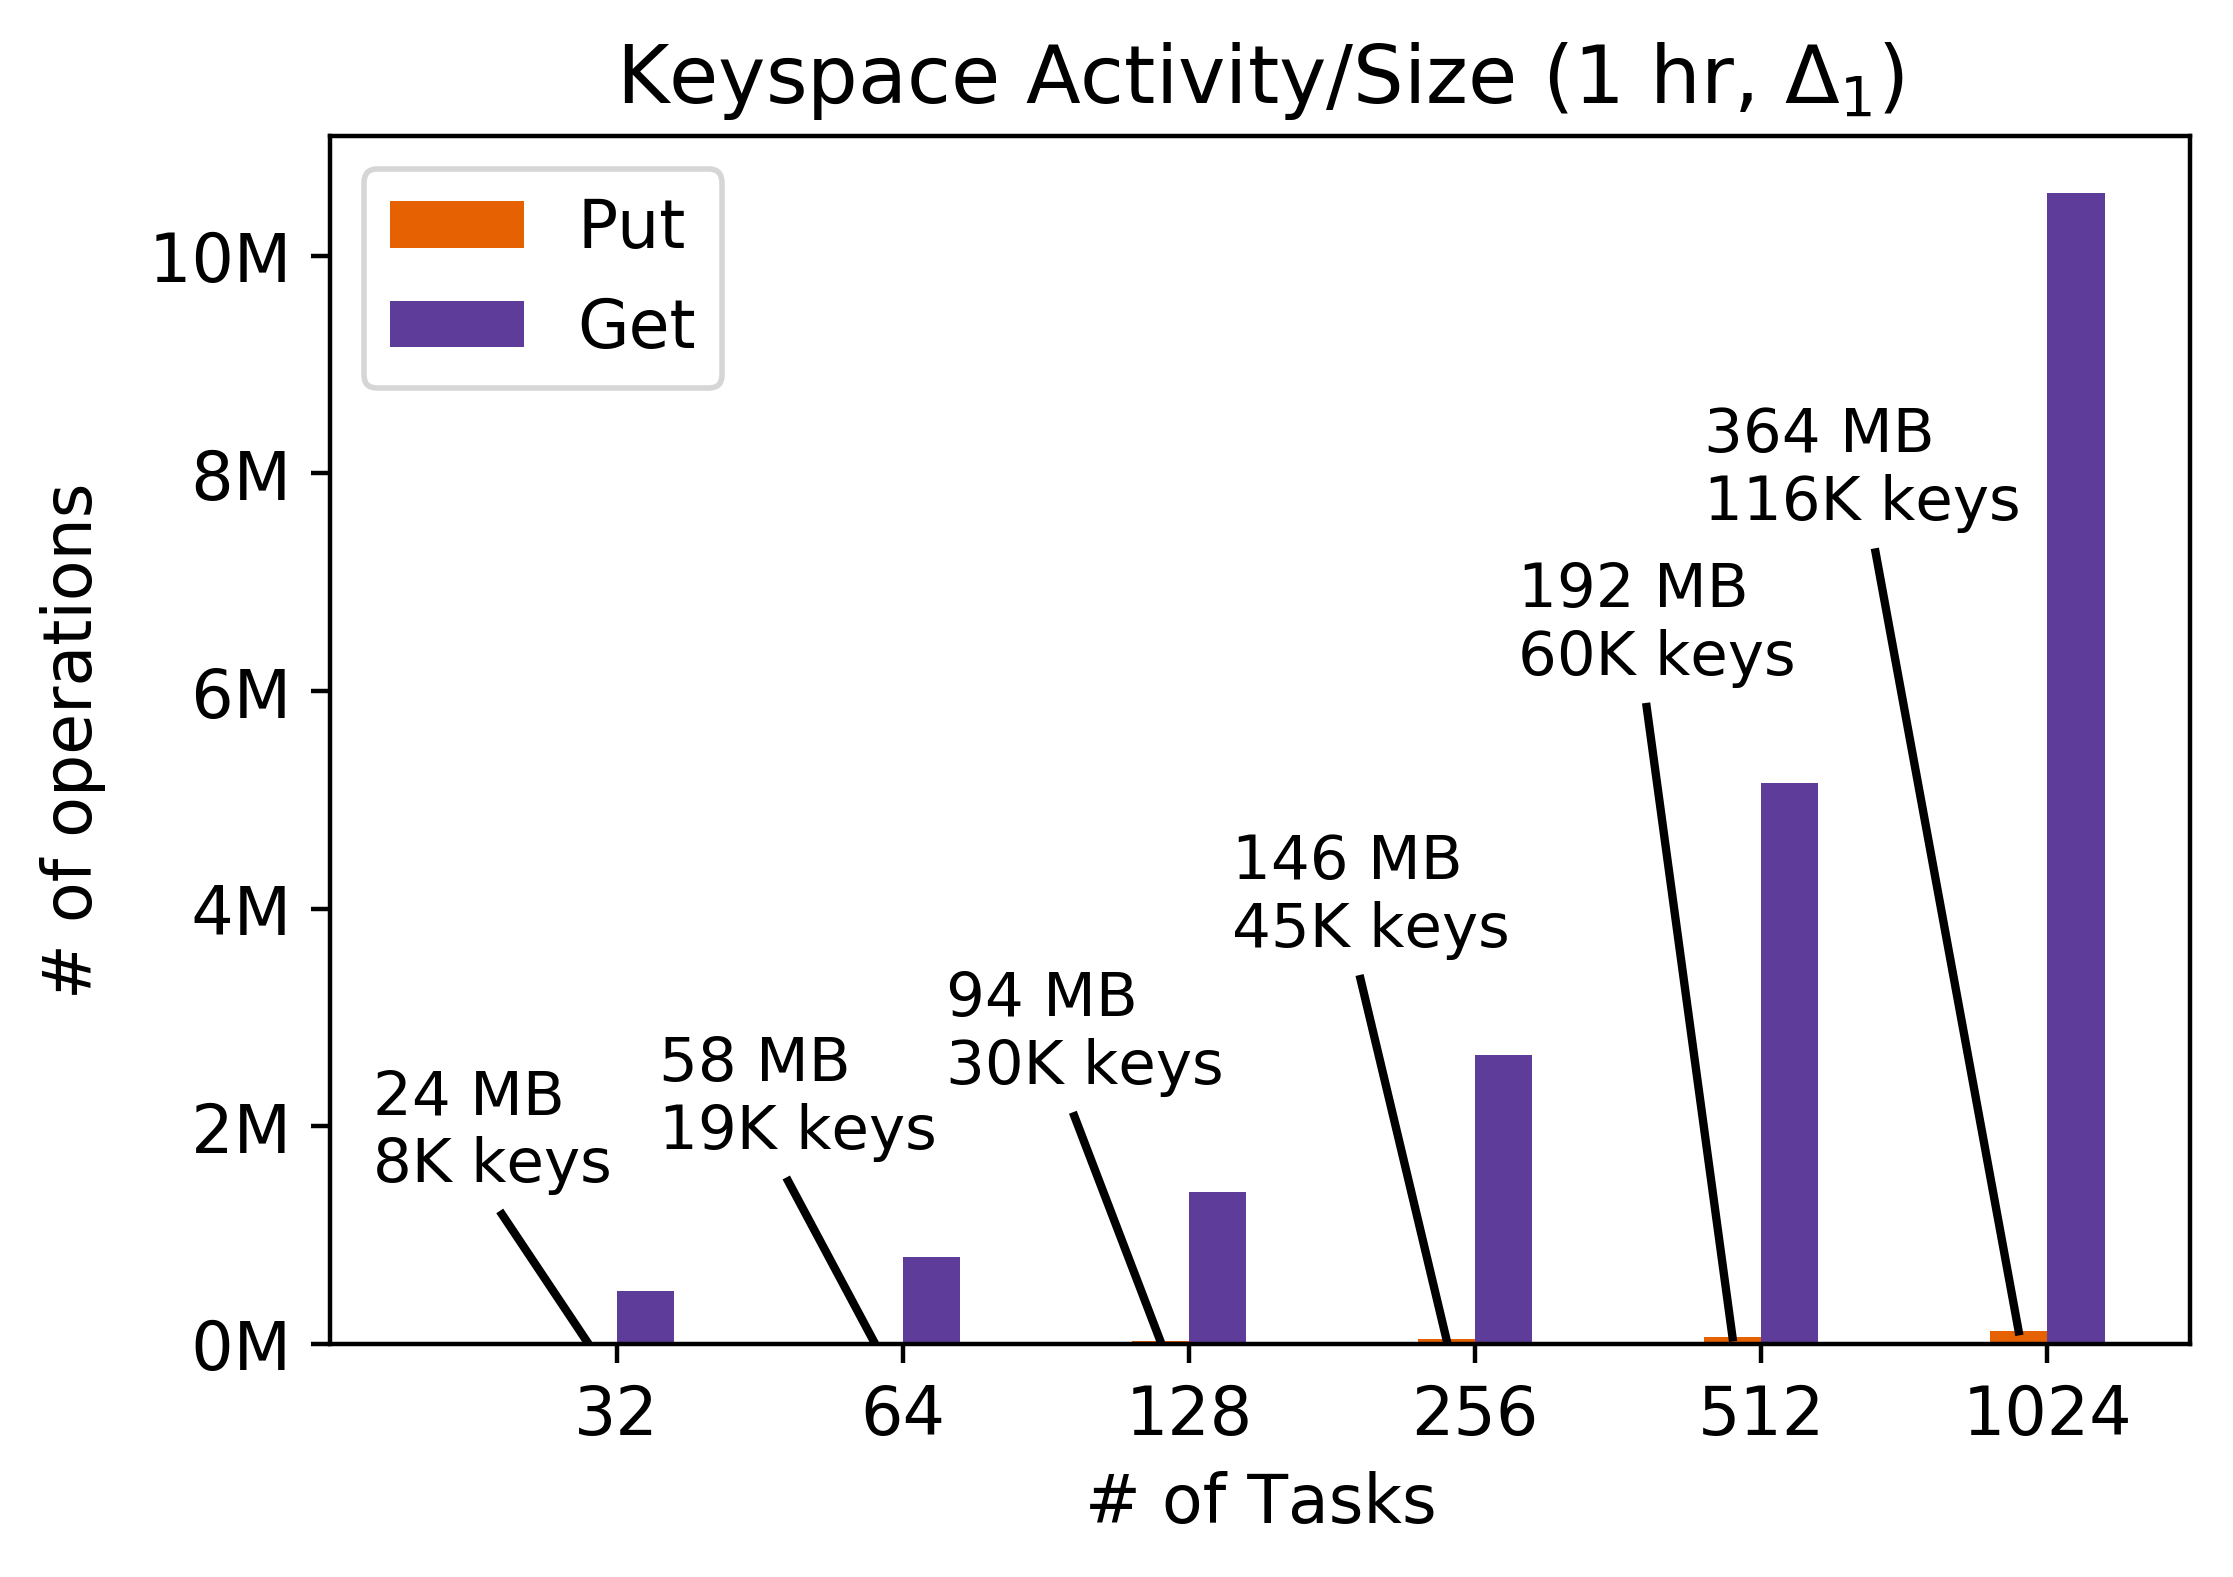
\includegraphics[width=0.5\textwidth]{./chapters/controlplane/parsplice/figures/methodology-keyspace.png}\\
  \caption{The keyspace is small but must satisfy many reads as workers
  calculate segments. Memory usage scales linearly, so it is likely that we will need
  more than one node to manage segment coordinates when we scale the system or jobs up.
  \label{fig:methodology-keyspace}}
\end{figure}

Our analysis shows that ParSplice accesses keys in a structured and predictable
way. The following 4 observations shape the policies we design later in the
paper.

\textbf{\underline{Scalability}} Figure~\ref{fig:methodology-keyspace} shows the
keyspace size (text annotations) and request load (bars) after a one hour run
with a different number of tasks (\(x\) axis). While the keyspace size and
capacity is modest the memory usage scales linearly with the number
of tasks, which is a problem if we want to scale to Trinitite's 3000 cores.
Furthermore, the size of the keyspace also increases linearly with the length
of the run.  Extrapolating these results puts an 8 hour run across all 100
Trinitite nodes at 8GB for one cache.  This memory utilization easily eclipses
the 3\% memory usage per node threshold we set earlier, even without factoring
in the usage from other workers.

\textbf{\underline{An active but small keyspace}}

The bars in Figure~\ref{fig:methodology-keyspace} show \(50-100\times\) as many
reads (\texttt{get()}) as writes (\texttt{put()}).  Tasks read the same key for
extended periods because the trajectory gets stuck in so-called superbasins
composed of tightly connected sets of states.  Writes only occur for the final
state of segments generated by tasks; their magnitude is smaller than reads
because the caches ignore redundant write requests. 

\begin{figure}[t]
  \noindent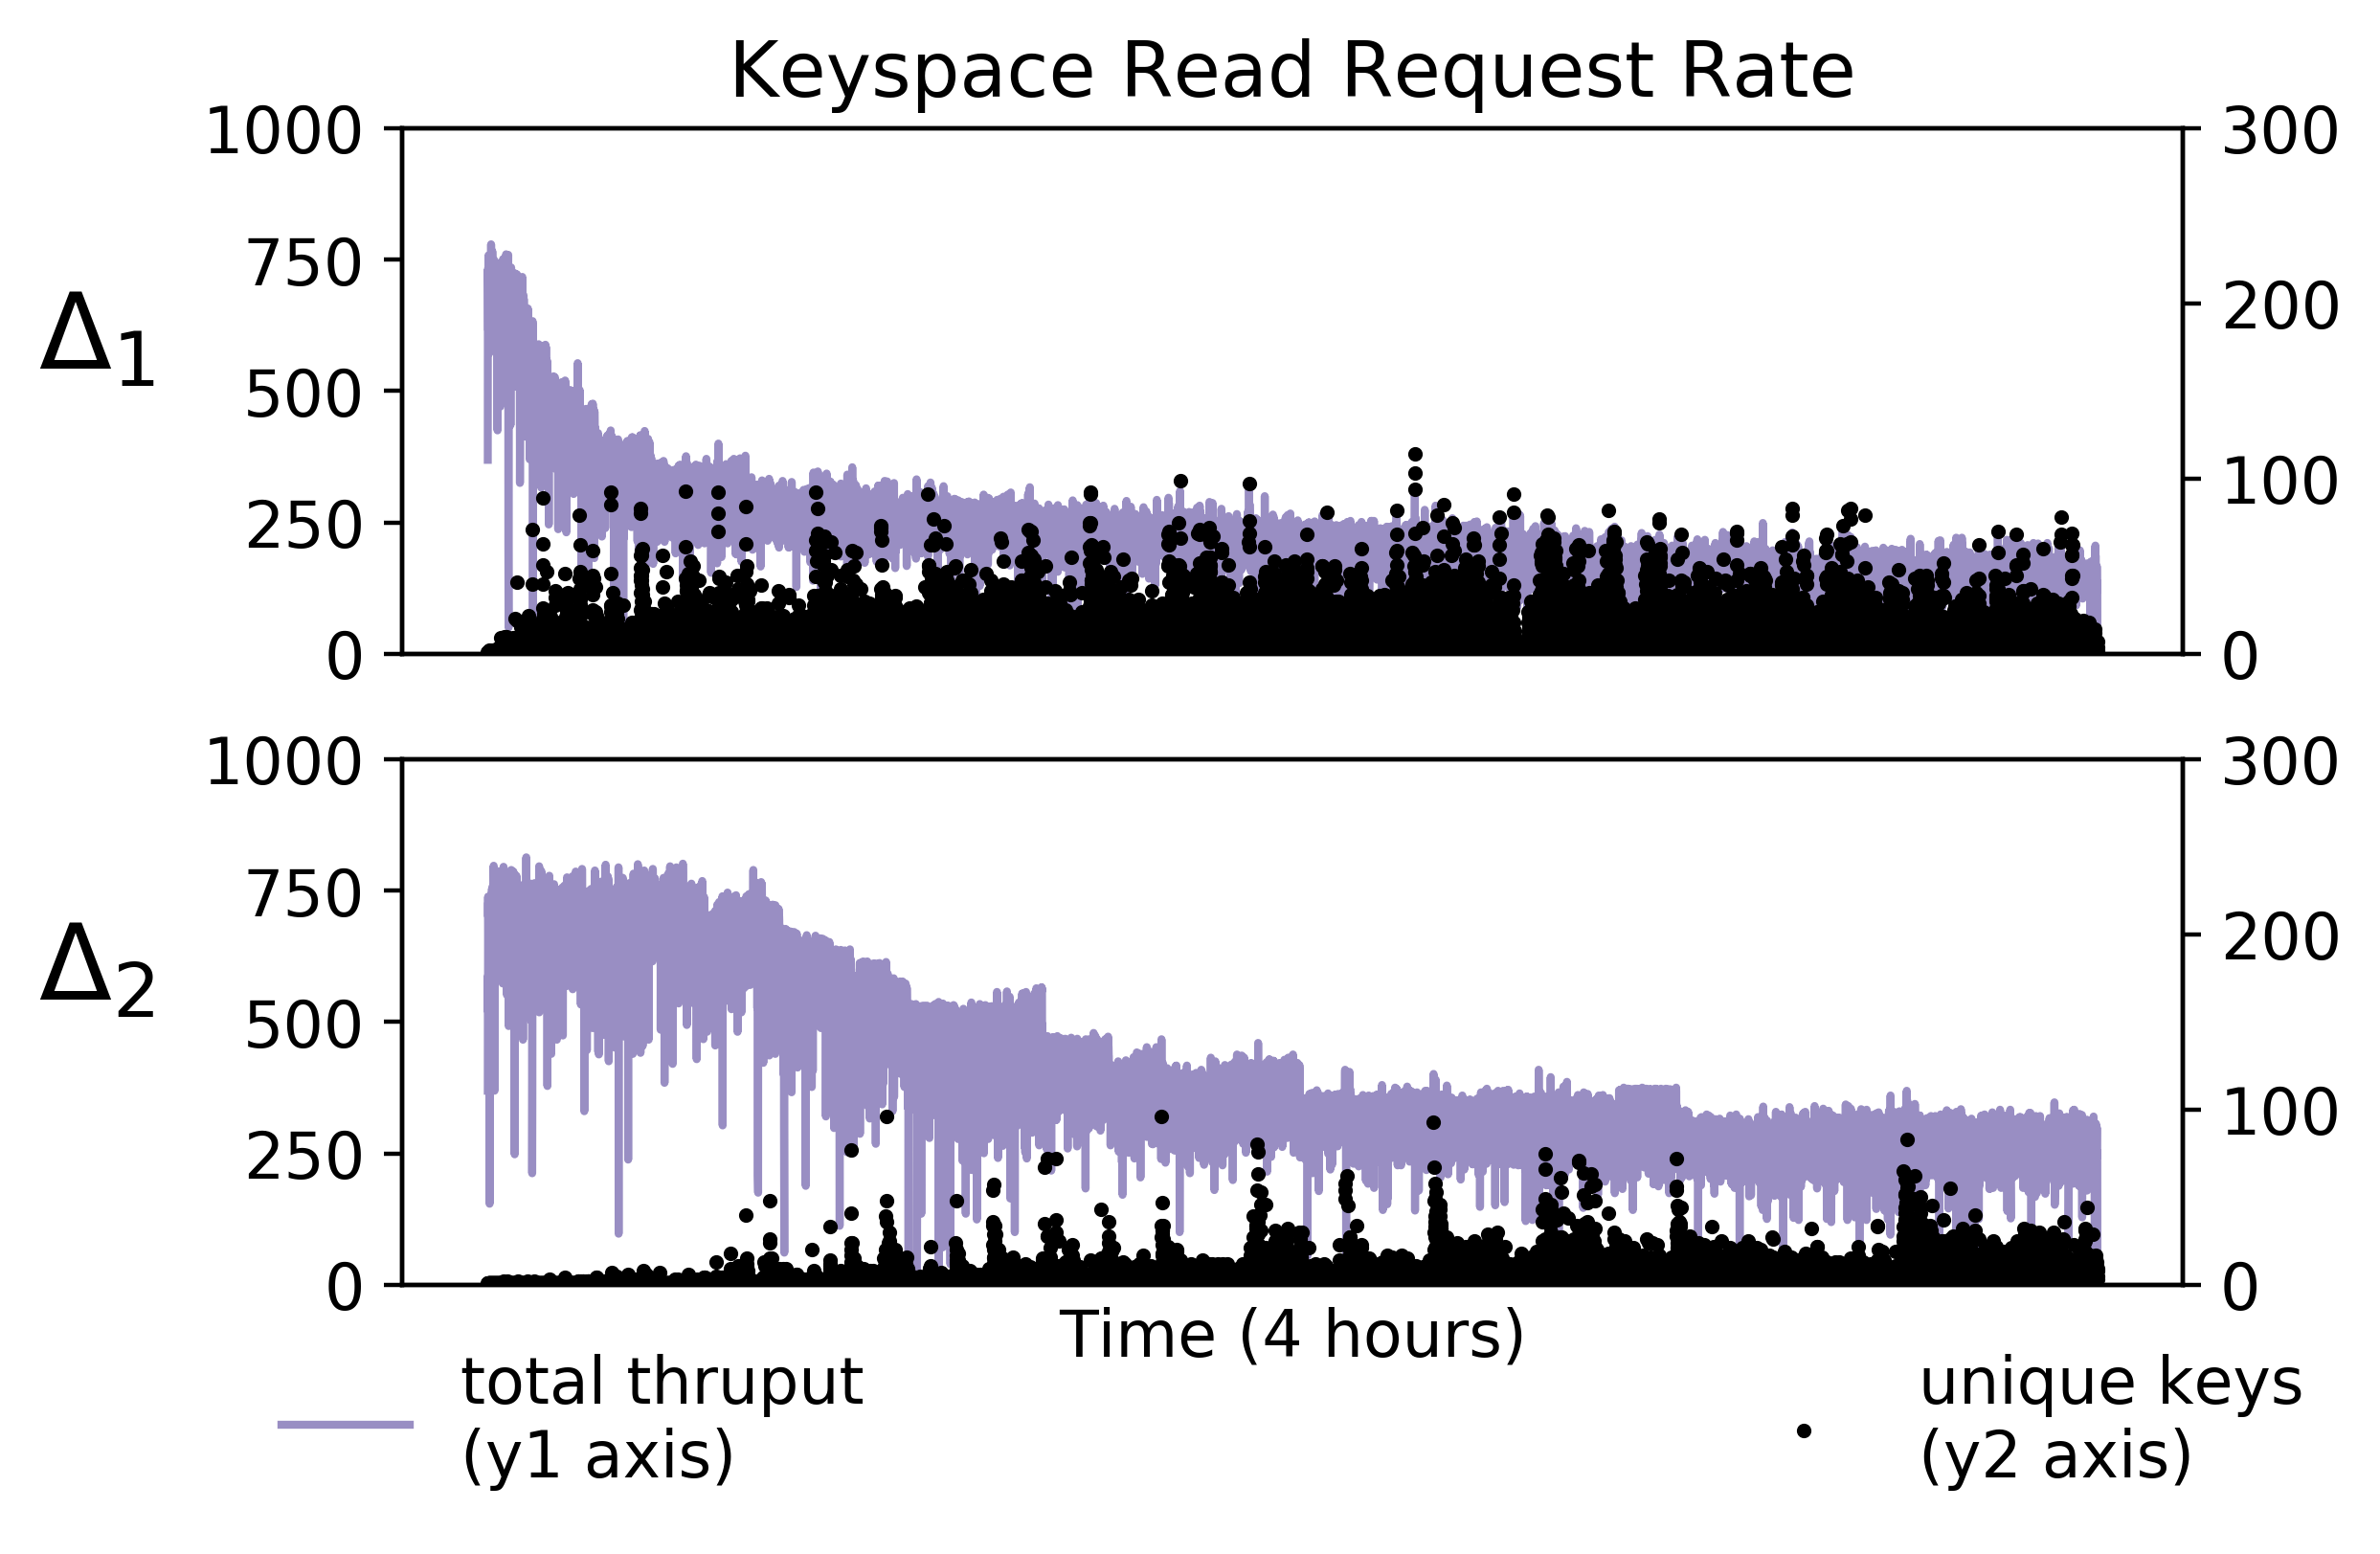
\includegraphics[width=0.5\textwidth]{./chapters/controlplane/parsplice/figures/motivation-regimes.png}\\
  \caption{Key activity for ParSplice starts with many reads to a small set of
keys and progresses to less reads to a larger set of keys.  The line shows the
rate that EOM minima values are retrieved from the key-value store (\(y1\)
axis) and the points along the bottom show the number of unique keys accessed in a 1
second sliding window (\(y2\) axis). Despite having different growth rates
(\(\Delta\)), the structure and behavior of the key activities are similar.
\label{fig:motivation-regimes}}
\end{figure}

\textbf{\underline{Initial conditions influence key activity}}
Figure~\ref{fig:motivation-regimes} shows how ParSplice tasks read key-value
pairs from the worker's cache for two different initial conditions of
\(\Delta\), which is the rate that new atoms enter the simulation.  The line is
the read request rate (\(y1\) axis) and the dots along the bottom are the
number of unique keys accessed (\(y2\) axis).  The access patterns for
different growth rates have temporal locality, as the reads per second for
\(\Delta_2\) look like the reads per second for \(\Delta_1\) stretched out
along the time axis.  The \(\Delta_1\) growth rate adds atoms every 100K
microseconds while the \(\Delta_2\) growth rate adds atoms every 1 million
microseconds. So \(\Delta_2\) has a smaller growth rate resulting in hotter
keys and a smaller keyspace.  Values smaller than \(\Delta_2\)'s growth rate or
a temperature of 400 degrees result in very little database activity because
state transitions take too long. Similarly, values larger than \(\Delta_1\)'s
growth rate or a temperature of 4000 degrees result in an equally meaningless
simulation as transitions are unrealistic.  

This figure demonstrates that small changes to \(\Delta\) can have a strong
effect on the timing and frequency with which new EOM minima are discovered and
referenced.  Trends also exist for temperature and number of workers but are
omitted here for space.  This finding suggests that we need a flexible policy
language and engine to explore these trade-offs.  

\begin{figure}[t]
  \noindent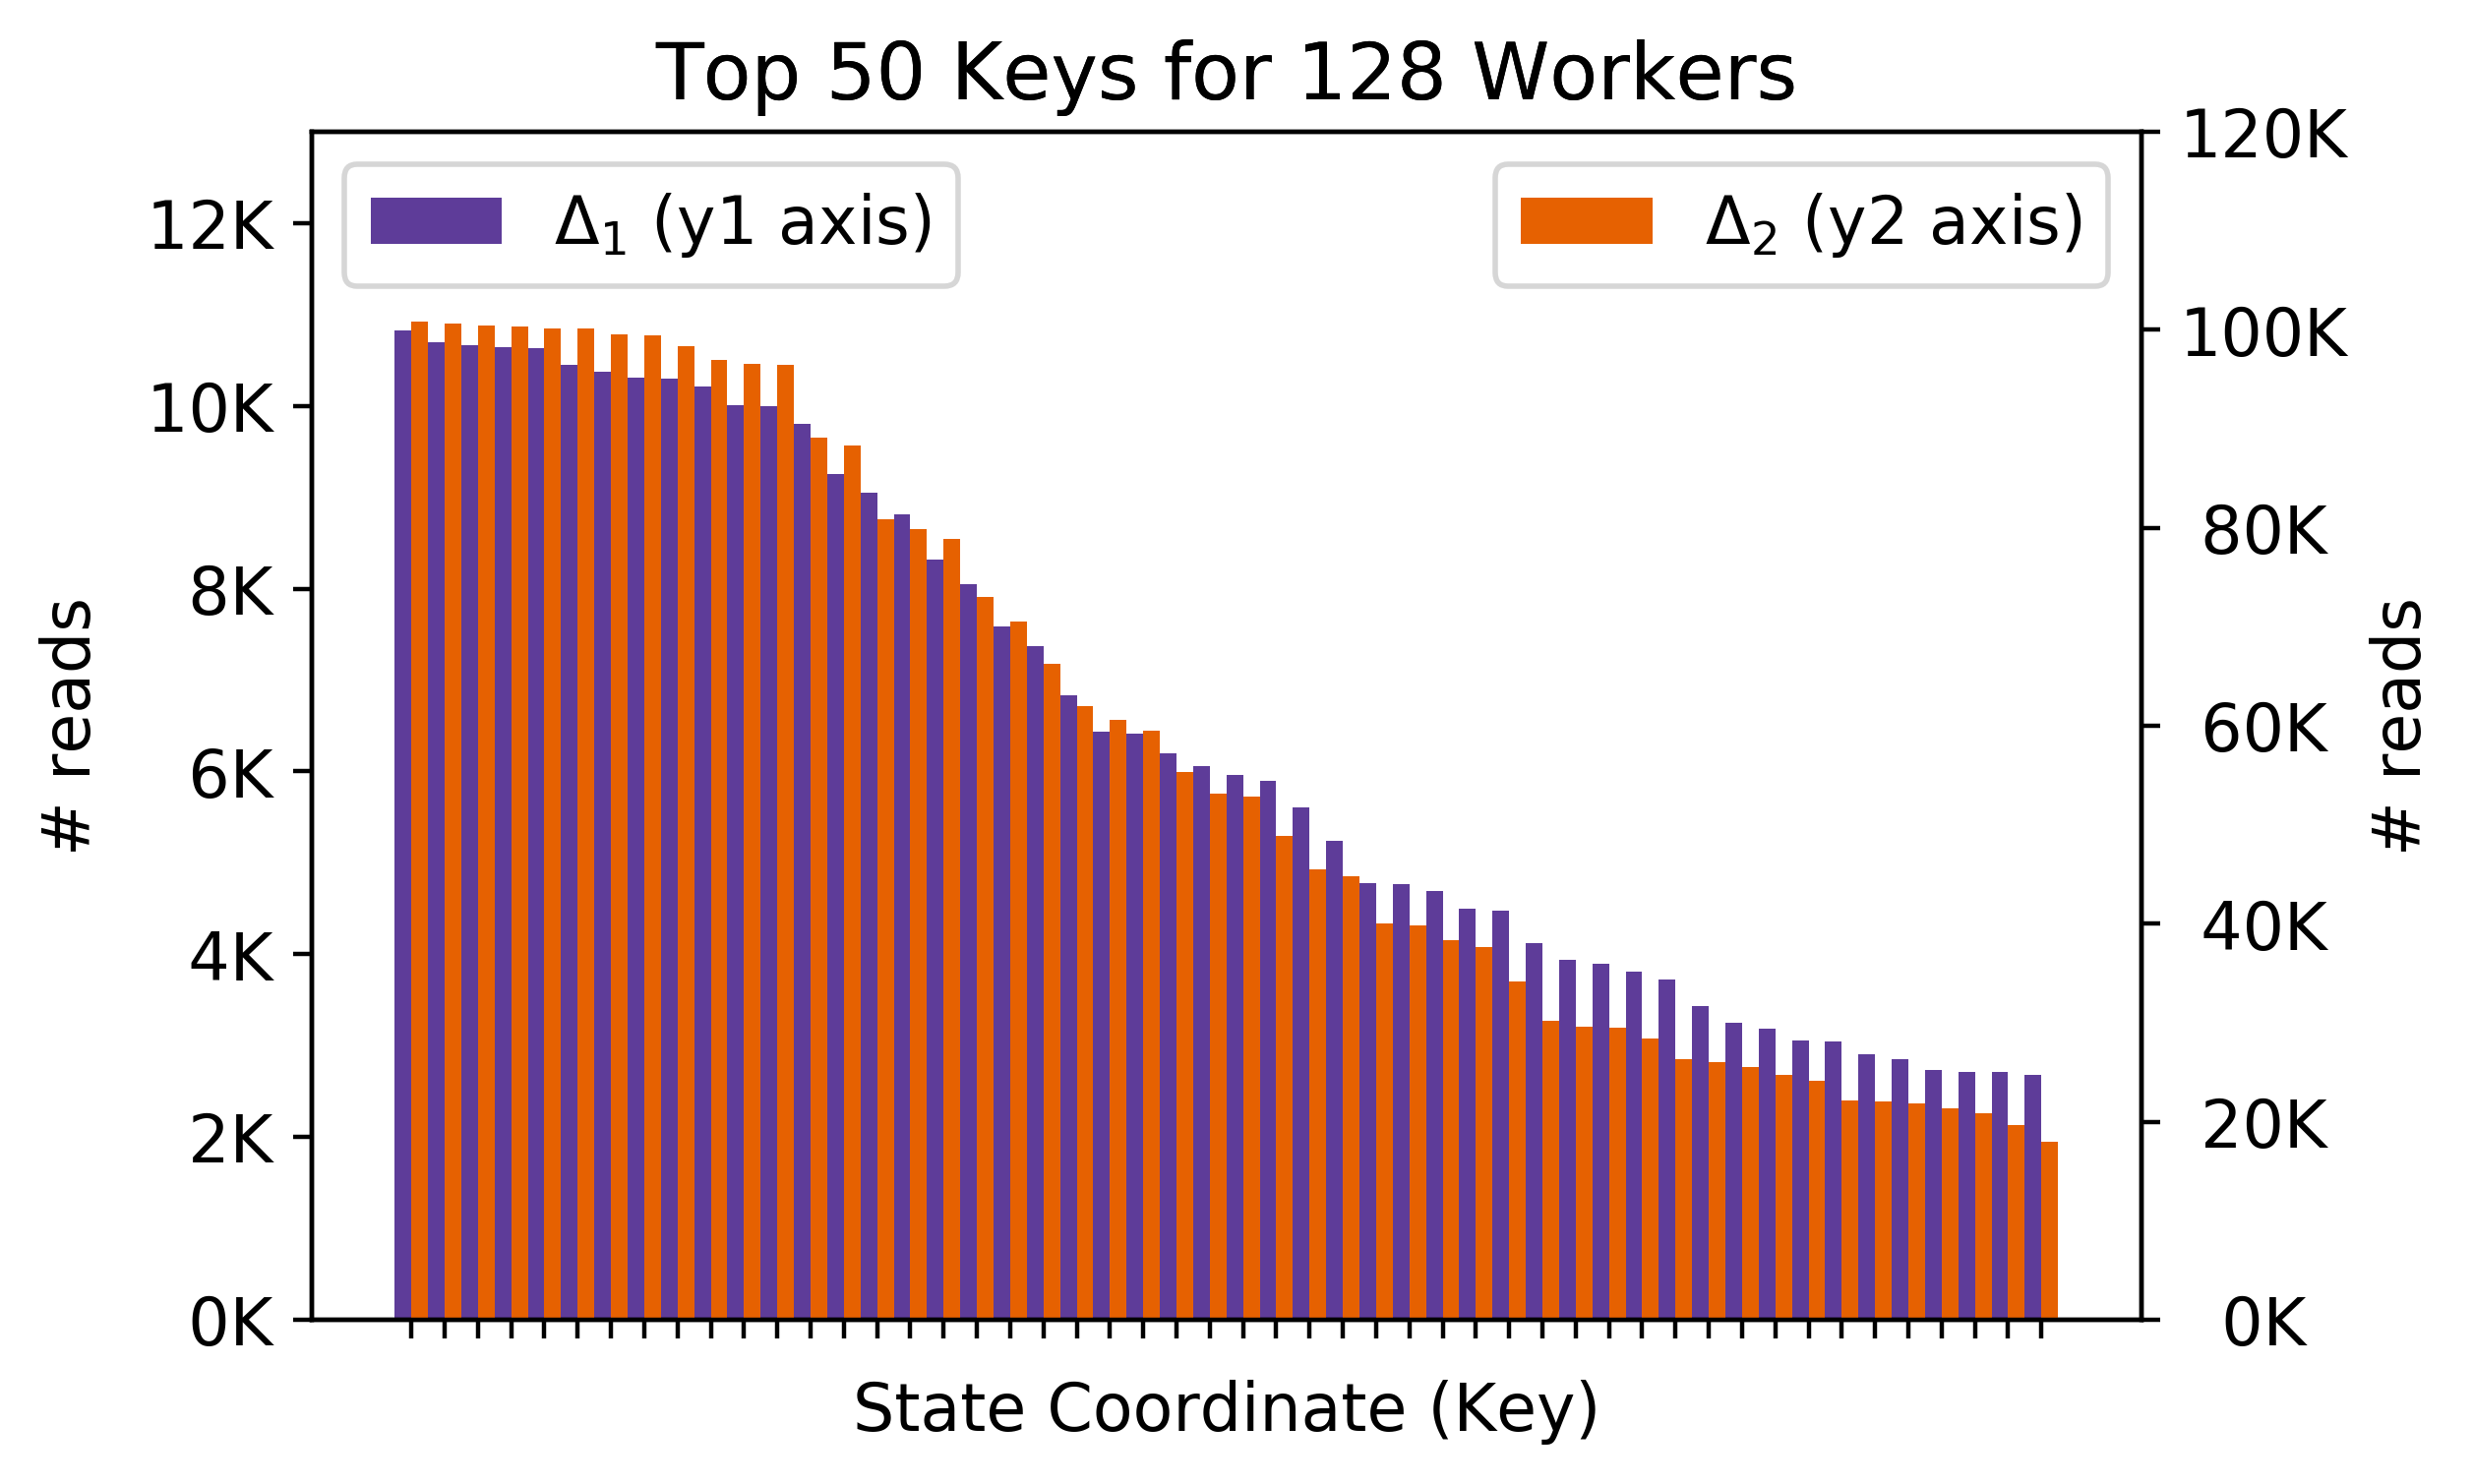
\includegraphics[width=0.5\textwidth]{./chapters/controlplane/parsplice/figures/methodology-keys.png}\\
  \caption{Over time, tasks start to access a larger set of keys resulting in
some keys being more popular than others.  Despite different growth rates
(\(\Delta\)), the spatial locality of key accesses is similar between the two
runs.  ({\it e.g.}, some keys are still read 5 times as many times others).
\label{fig:methodology-keys}}
\end{figure}

\textbf{\underline{Entropy increases over time}} The reads per second in
Figure~\ref{fig:motivation-regimes} show that the number of requests decreases
and the number of active keys increases over time.  The number of read and
write requests are highest at the beginning of the run when tasks generate
segments for the same state, which is computationally cheap (this motivates
Section~\S\ref{sec:arch-specific}).  The resulting key access imbalance for the
two growth rates in Figure~\ref{fig:motivation-regimes} are shown in
Figure~\ref{fig:methodology-keys}, where reads are plotted for each unique
state, or key, along the \(x\) axis. Keys are more popular than others (up to
\(5\times\)) because worker tasks start generating states with different
coordinates later in the run.  Figure~\ref{fig:methodology-keys} also shows that the
number of reads changes with different initial conditions (\(\Delta\)), but
that the spatial locality of key accesses is similar ({\it e.g.}, some keys are
still \(5\times\) more popular than others).
